

\chapter{General context}
The number of Canadians suffering from Alzheimer's disease (AD) is rapidly increasing, with tremendous social and economic impact. Despite the emergence of promising drugs, the recent clinical trials with demented patients have failed. Dementia however comes very late in the development of the disease, at a stage where the degeneration of neural tissues has likely gone beyond repair. In order to be efficient, therapies should be initiated in the decades predating dementia, in a preclinical stage where patients experience no or very mild symptoms (see chapter $1.1$). There are unfortunately no biomarker(s) that are currently predictive of AD in this preclinical stage, and could help identify the individuals that could benefit from such interventions. A promising technique is resting-state functional magnetic resonance imaging (rs-fMRI), which may be able to capture the early synaptic dysfunction seen in AD (see chapter $1.2$). I order to be able to apply statistical analysis and machine learning methods we 
need to preprocess the data to remove as much as possible the effect of various artefacts (hardware and physiological). The preprocessing reduces the variability of the data and therefore provides more relevant and discriminative features (see chapter $1.3$). In order to further improve the statistical power of there analysis, multiple academic groups are collaborating to pool their dataset to increase the sample size of the study. Unfortunately the gain in sample size comes with a new source of variability introduced by the multicentric acquisition. Site-specific MRI set-ups may bias the fMRI measures, and I am thus developing procedures for inter-site normalization. Account for these sources of variance are important since they may bias the predictive potential of rs-functional connectivity in a multi-site, in line with this last assumption we want to quantify the robustness of the feature selection and classifier to multi-site acquisition (see chapter $1.4$).

With the objective of extracting meaningful information that could be used as biomarkers we are using connectivity measures usually based on the correlation of spontaneous fluctuations in neurovascular activity from pairs of brain regions, which have been shown to be sensitive to the development of the disease (see chapter $1.5$). However, with about $10^4$ recording sites in the gray matter and close to no knowledge on the early brain dysfunction in AD, there is an overwhelming number of $10^7$ possible connections to examine as a potential diagnostic we will therefore focus on the feature selection procedure and the stability of those selections in order to have consistent and sparse predictive features discriminative of the disease(see chapter $1.6$). The main outcome of this project will be a prediction pipeline for the data-driven identification of AD biomarkers in resting-state fMRI.

\section{Alzheimer's disease} Alzheimer's disease (AD) is a major neurodegenerative disorder characterized by cognitive and intellectual deficits and behavioural changes without a known cause or an effective treatment. It gradually destroys a patient's memory and ability to reason, make judgments, communicate and carry out daily activities \citep{Jeong2004}. With the aging of the population worldwide, this disorder has attracted much attention. Evidence from clinical elderly individuals suggests that the pathophysiological process of AD begins years, if not decades, before the diagnosis of clinical dementia \citep{Morris2005}. The clinical disease stages of AD are divided into three phases described by Jack and colleagues \cite{Jack2010}. 

\textit{First is a pre-symptomatic phase in which individuals are cognitively normal but some have pathological changes in AD. Second is a prodromal phase of AD, commonly referred to as mild cognitive impairment (MCI) \citep{Petersen2004}, which is characterised by the 
onset of the earliest cognitive symptoms (typically deficits in episodic memory) that do not meet the criteria for dementia. The severity of cognitive impairment in the MCI phase of AD varies from early manifestation of memory dysfunction to more widespread dysfunction in other cognitive domains. The final phase in the evolution of AD is dementia, defined as multi-domain impairments that are severe enough to result in loss of function} \citep{Jack2010}.

The use of biomarker for the early diagnostic of pathologies has a long history, with many studies showing the feasibility of using AD biomarker to predict conversion from MCI to AD. These studies show that individuals on the course of developing AD can be identified earlier in the course of the disease by using the MCI stage with the addition of imaging and cerebrospinal fluid (CSF) biomarkers to enhance diagnostic specificity \citep{Chetelat2003,Jack1999,Yuan2009,Mattsson2009}. 
It could be possible to diagnose AD after the exclusion of other forms of dementia, although a formal diagnostic can only be made after a post-mortem evaluation of the brain tissue \citep{McKhann1984}. This is one of the reasons why MRI based analysis and diagnostic tools are currently a hot topic in clinical neuroscience research.

The currently dominant hypothesis in the field for the chain of events in AD pathophysiology is the $\beta$-amyloid (A$\beta$)-cascade hypothesis. It suggests that interstitial A$\beta$ proteins exert a toxic effect on surrounding neurons and synapses by forming plaques, thereby disturbing their function \citep{Hardy2002,Shankar2008}. Moreover, recent research study suggests that, prior to neuronal death resulting in brain atrophy, disruption of functional connectivity may arise in response to an unknown systemic problem and represent an early outcome of A$\beta$ proteins plaque formation in AD \citep{Sheline2013}. Atrophy is the result of neuronal death and is measures in vivo using structural MRI measuring the thickness of the gray matter on the cortex (also called cortical thickness). Already in the stage preceding aggregation of A$\beta$ fragments into amyloid plaques, there is a dysfunction of synaptic transmission in many brain regions due to dimers and monomers from the A$\beta$ cascade \citep{
dAmelio2012}. As illustrated in \cite{Sperling2011} a viable hypothesis is that fMRI precedes the structural changes as well as clinical symptoms and is believed to start in the preclinical phase of the disease.


\begin{figure}[H]
\begin{center}
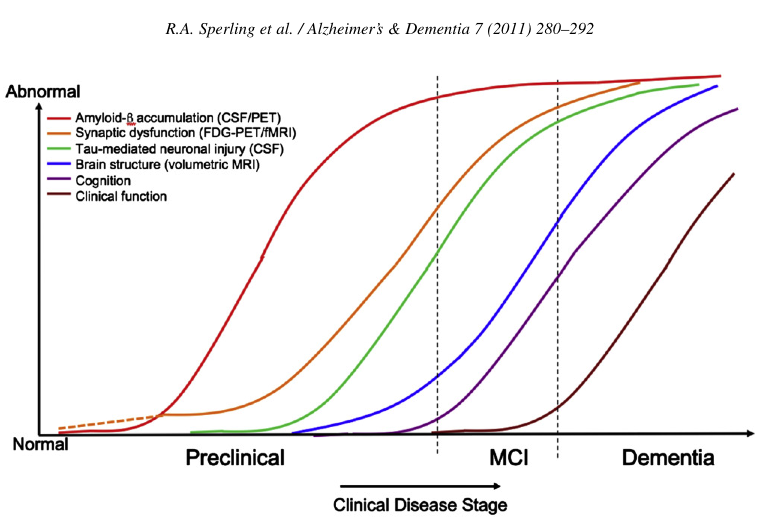
\includegraphics[width=\linewidth]{../figures/ad_progression.png}
\end{center}
\caption[Biomarker model of Alzeimer's disease]
{Hypothetical model of dynamic biomarkers of the AD expanded to explicate the preclinical phase: A$\beta$ as identified by cerebrospinal fluid A$\beta$42 assay or PET amyloid imaging. Synaptic dysfunction evidenced by fluorodeoxyglucose (F18) positron emission tomography (FDG-PET) or functional magnetic resonance imaging (fMRI), with a dashed line to indicate that synaptic dysfunction may be detectable in carriers of the 34 allele of the apolipoprotein E gene before detectable A$\beta$ deposition. Neuronal injury is evidenced by cerebrospinal fluid tau or phospho-tau, brain structure is evidenced by structural magnetic resonance imaging. Biomarkers change from normal to maximally abnormal (y-axis) as a function of disease stage (x-axis). The temporal trajectory of two key indicators used to stage the disease clinically, cognitive and behavioral measures, and clinical function are also illustrated. Figure from \cite{Sperling2011}.}
\label{fig_biomarker_model}
\end{figure}


\section{Overview of functional magnetic resonance imaging} In functional magnetic resonance imaging (fMRI), the acquisition process is slightly different than for the anatomical MRI acquisition. fMRI uses the principle of the relaxation of hydrogen nuclei, by using specific fMRI sequences consisting in $T2*$ weighted acquisitions that are sensitive to local distortions of the magnetic field. Particularly, deoxyhemoglobin (a form of hemoglobin without oxygen) will create such local distortions of the magnetic field, since it is a paramagnetic molecule (positive magnetic susceptibility) \citep{Ogawa1990}. The data acquired using fMRI rely on the hypothesis that areas showing decreased deoxyhemoglobin concentration are due to sustained brain activity. Following neuronal activity, neurons require energy to restore the electrical and ionic concentration balance across the cell membrane. One mechanism to generate this energy is the glucose oxidative metabolism, which requires the delivery of oxygen and glucose by 
the blood on the site where brain activity takes place \citep{Ogawa1990}
. Initially, fMRI was thought to be a good technique to measure the cerebral metabolic rate of oxygen, since the new blood rushing in causes a proportional effect on the venous-end, resulting in a decrease in deoxyhemoglobin concentration, and thus an increase in fMRI signal. The concentration of deoxyhemoglobin actually depends mainly on three factors or phenomena: metabolic rate of oxygen consumption, cerebral blood volume (CBV) and cerebral blood flow (CBF) \citep{Hoge1999}. As a result, the fMRI signal is the outcome of competing effects following neuronal activity
%. CBF augmentation tends to decrease the deoxyhemoglobin concentration due to an increase in the oxygenated blood (resulting in a increase fMRI signal). While an increase in cerebral metabolic rate of oxygen and CBV tends to increase deoxyhemoglobin within the tissue at the vicinity of the neural activity, resulting in a decrease fMRI signal due to the paramagnetic properties of deoxyhemoglobin. The fMRI signal is the result of competing effects 
 and fortunately these effects do not cancel out, allowing the detection of a net signal increase. We call the interrelation of theses effects the blood oxygenation level dependent (BOLD) effect.

\begin{figure}[H]
\begin{center}
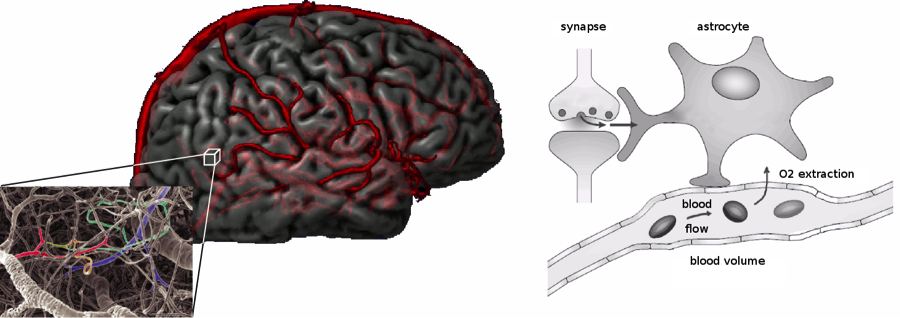
\includegraphics[width=\linewidth]{../figures/bold.png}
\end{center}
\caption[Schematic of the BOLD effect]
{Representation of the brain and its vasculature (on the left) and a schematic view of the interaction between the effect of neuronal activity on local changes in blood oxygenation signal (BOLD) (on the right) (adapted from \cite{Heeger2002}).}
\label{fig_bold}
\end{figure}

\section{Preprocessing}Normalization of the data is crucial to obtain a consistent and accurate classifier \citep{Kotsiantis2007}. Therefore a particular attention is place on the correction and normalization procedure applied to the rs-fMRI data used in this study. A series of standard preprocessing steps is usually applied in an attempt to correct for various artefacts that would perturb the subsequent analysis. The BOLD effect associated with neuronal activity generally results in a relatively small fluctuation of the MR signal. Many factors can influence this signal. Among them,  the physiological activity associated mainly with respiration, cardiac pulsations and patient's motion are major contributors to the noise and are spatially spread everywhere within the brain volume. These sources of noise result in large correlations between BOLD signals of distant voxels. An other factor is the fact that we need a form of spatial normalization of the individual brains in order to perform analysis across 
subjects (due to anatomical variance among subjects), this spatial normalization (coregistration of the individual brains with an reference template) is necessary but can potentially be an other source of confound. 
%Therefore, analyzing directly raw rs-fMRI data with seed-based connectivity or with a data driven technique (like ICA or clustering) will more likely result in the identification of noise related structures spread everywhere within the brain.
Therefore, preprocessing methods were designed in an attempt to remove specifically the so-called structured noise and motion artefacts from the raw fMRI data. A schematic representation of the preprocessing pipeline can be seen in Figure \ref{fig_preprocessing}.

\begin{figure}[H]
\begin{center}
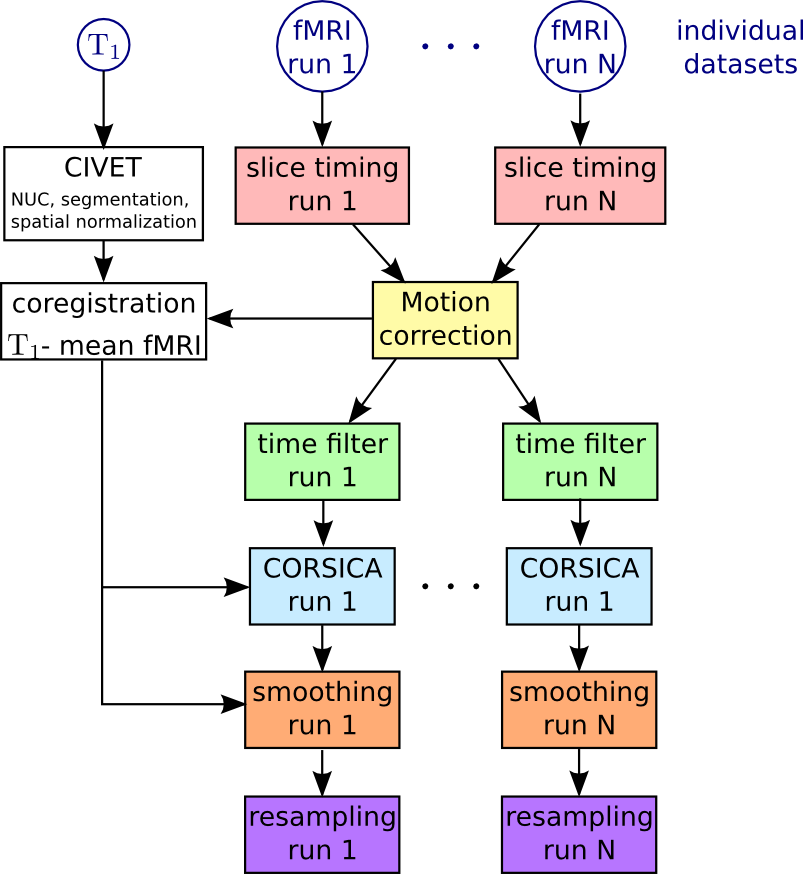
\includegraphics[scale=0.7]{../figures/fig_flowchart_fmri_preprocess.png}
\end{center}
\caption[Schematic of the preprocessing]
{Schematic of the preprocessing pipeline including spatial and functional normalization (NIAK preprocessing pipeline \footnote{\url{http://www.nitrc.org/projects/niak/}}).}
\label{fig_preprocessing}
\end{figure}

The basic steps are as follow: (1) correction for slice timing differences due to delay in acquisition sampling; (2) rigid-body motion estimation for within and between runs, motion correction operates by selecting one functional volume as a reference to align all other functional volumes. Most head motion algorithms describe head movement by 6 parameters, three translation (displacement) parameters and rotation parameters and are appropriate to characterize motion of rigid bodies (see Figure \ref{fig_motion_estimation}); (3) Coregistration of the functional data in a reference space; (4) resampling of the functional data in the stereotaxic space (references brain used as a common space between subjects); (5) regression of confounds in order to remove spatially structured noise on the fMRI 
time-series. The confounds are the slow time drift, high frequency noise signal, motion parameters, the average signal white matter as well as the average signal of the ventricles (containing cerebrospinal fluid CSF a frequent source of noise and artefact). Some groups have suggested that these corrections are not sufficient to remove motion artefact and propose some additional corrective procedure (detailed in Chapter 2); and (6) the spatial smoothing is usually applied using a Gaussian blurring kernel to improve signal to noise ratio (SNR), improved validity of the statistical tests by making the error distribution more normal and finally reduce anatomical and functional variations between subjects \citep{Worsley1995,Mikl2008}. %There is however a few drawbacks from this procedure like the reduction of spatial resolution of the data, edge artefact from smoothed brain voxels with non-brain voxels which might result in hypoactivation of the regions in question.

\begin{figure}[H]
\begin{center}
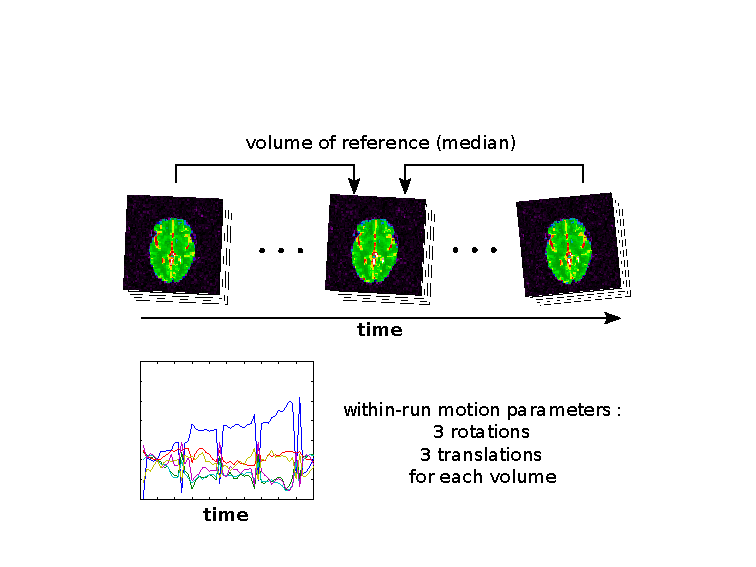
\includegraphics[scale=0.9]{../figures/motion_estimation.pdf}
\end{center}
\caption[Motion estimation]
{Motion estimation based on rigid-body motion estimation of the functional volumes, the procedure provide 6 motion parameters for each volume (3 translation and 3 rotation) Schematic of the preprocessing pipeline including spatial and functional normalization (from NIAK preprocessing pipeline \footnote{\url{http://www.nitrc.org/projects/niak/}}).}
\label{fig_motion_estimation}
\end{figure}



\section{Multi-site}
In most experiments conducted in neuroimaging, the main factors that influence power are: (1) the size of the effect, determined by the difference of the mean connectivity of one group versus a control group and the variability of this difference across subjects and groups; (2) the probability of rejecting the null hypothesis when it is true; and (3) the sample size, i.e. the number of subjects in the study \citep{Desmond2002}. This last factor is usually the only one controlled by the investigator, hence why an increasing number of researchers share multicentric, sometimes multiprotocol, data suitable to statistical analysis. In research it is very difficult to obtain a grant large enough to scan a cohort larger than ~80 subjects, therefore researcher and consortium initiatives have started to pool their resources together to make initiative composed of publicly available large cohorts of subjects like the 1000 functional connectome \citep{Biswal2010}, ADNI \citep{
Mueller2005}, among 
others. In clinical trial the justification for multicentric acquisition is more of a logistical one then a financial reason; they need to recruit a large amount of subject in a short period of time. In order to achieve this goal they mandate the recruitment to multiple clinical centers across the globe which accelerate the evaluation time of a drug. Although these centers may be similar by their scanner protocols, scanners will have difference in their software version, specific add-on to the scanners, and, most importantly, vendors (even field strength may differ in some cases). Unfortunately between studies, MR acquisition methodologies are among the most commonly cited sources of measurement variation \citep{Friedman2006}. This is why it is important to assess if multi-site resting-state connectivity analysis are feasible (we can combine the data from multiple sources while introducing a reasonable amount of variance which is still acceptable to detect effects in the data) and what corrective measure on 
the data should be applied to reduce the bias introduced by multi-site analysis. Among the factor of variability across sites, we can list the following 3 categories described in \citep{Yan2013a}:


\textit{
\begin{enumerate}
\item Acquisition-related variations:
\begin{enumerate}
\item Scanner make and model \citep{Friedman2006}
\item Sequence type (spiral vs. echo planar; single-echo vs. multi-echo) \citep{Klarhoefer2002}, parallel vs. conventional acquisition \citep{Feinberg2010} \citep{Lin2005}
\item Coil type (surface vs. volume, number of channels, orientation).
\item Acquisition parameters: repetition time, number of repetitions, flip angle, echo time, and acquisition volume (field of view, voxel size, slice thickness/gaps, slice prescription) \citep{Friedman2006a}.
\end{enumerate}
\item Experimental-related variations: 
\begin{enumerate}
\item Participant instructions \citep{Hartstra2011}, eyes-open/eyes-closed \citep{Yan2009} \citep{Yang2007}, visual displays, experiment duration \citep{Fang2007} \citep{VanDijk2010}.
\end{enumerate}
\item Environment-related variations: 
\begin{enumerate}
\item Sound attenuation measures \citep{Cho1998} \citep{Elliott1999}.
\item Attempts to improve participant comfort during scans (e.g., music, videos) \citep{Cullen2009}.
\item Head-motion restraint techniques (e.g., vacuum pad, foam pad, bite-bar, plaster cast head holder) \citep{Edward2000} \citep{Menon1997}.
\item Room temperature and moisture \citep{Vanhoutte2006}.
\end{enumerate}
\end{enumerate}
}


In 2009, the publicly released 1000 Functional Connectomes Project (FCP) and International Neuroimaging Data-sharing Initiative (INDI) provided a glimpse of the variability in imaging methodologies employed by the neuroimaging field. The dataset includes rs-fMRI samples independently collected at imaging sites around the world. A noteworthy aspect of this dataset is the variation in almost every parameter of the imaging acquisition methodologies, while the majority of subject-related variables are not reported (due in most cases, to the fact that they were not thoroughly recorded). 
Despite justifiable scepticism, feasibility analyses demonstrated that meaningful explorations of the aggregate dataset, composed of 24 imaging sites for a grand total of 1093 subjects, could be performed \citep{Biswal2010}. Although no explicit correction for multi-site variability was used, they only use global signal correction (GSC) to normalize subjects which may introduce anti-correlation in the data \citep{Fox2009, Murphy2009, Saad2012, Carbonell2014, Power2014}. After accounting for site-related differences, the analysis showed brain-behaviour relationships with phenotypic variables such as age, gender, and diagnostic label, and confirmed a variety of prior hypotheses \citep{Biswal2010, Fair2012, Tomasi2010, Zuo2012}. While encouraging, many uncontrolled and unknown factors in the 1000 FCP remain a source of concern, as they spread beyond simple site effects and can limit the datasets utility as highlighted by \cite{Yan2013}.
An other compelling proof of multi-site bias is the study reported by \cite{Nielsen2013} where they did an analysis on a single site dataset and a multi-site dataset of subject with autism and concluded that the multi-site autism study classification accuracy significantly outperformed chance but was much lower for multi-site prediction than for previous single site results \citep{Nielsen2013}. We therefore need to keep in mind that the site effect must be taken in account in the analysis or we may reduce our detection power.


\section{Resting-state connectivity}
Resting-state (RS) functional connectivity captures slow fluctuations of hemodynamic activity without performing any task. These temporal fluctuations can be monitored using the signal measured with fMRI. The first study that introduced the concept of resting state functional connectivity was the one of \cite{Biswal1995}. By performing a task activation response to bilateral left and right finger tapping, Biswal and colleagues were able to activate the corresponding motor areas on the cortex. In a second analysis, they considered one of the area activated during the task as a seed region for a seed-based analysis in resting-state condition. Seed-based analysis consists in detecting temporal correlation between the signal of the predefined seed area and the time course of all the voxels of the brain. Using this seed-based analysis, they found RS correlations between similar brain regions than the ones involved during the task. A more recent review done 
by \cite{Fox2007} illustrated in Figure \ref{fig_rs} show the ability to identify the complete sensorimotor network using only the bold signal from a small region in that network. 

\begin{figure}[H]
\begin{center}
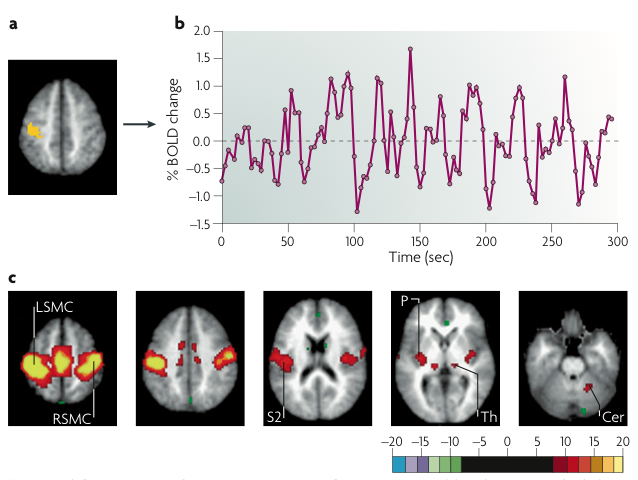
\includegraphics[width=\linewidth]{../figures/resting_state.png}
\end{center}
\caption[Resting-state correlation maps]
{Generation of resting-state correlation maps. a) Seed region in the left somatomotor cortex (LSMC) is shown in yellow. b) Time course of spontaneous blood oxygen level dependent (BOLD) activity recorded during resting fixation and extracted from the seed region. c) Statistical z-score map showing voxels that are significantly correlated with the extracted time course. Their significance was assessed using a random effects analysis across a population of ten subjects. In addition to correlations with the right somatomotor cortex (RSMC) and medial motor areas, correlations are observed with the secondary somatosensory association cortex (S2), the posterior nuclei of the thalamus (Th), putamen (P) and cerebellum (Cer) \citep{Fox2007}.}
\label{fig_rs}
\end{figure}

In resting-state acquisition, no task is performed during the scan; the subject is instructed to rest with his eyes open or closed, as opposed to the task-based acquisition where the subject has to perform a specific task. These early results from Biswal et al. suggest that it is possible to identify the functional organization of different structures without doing any specific task, just by looking at spontaneous fluctuations in brain activity. Several studies have demonstrated that patterns extracted from temporal correlations of rs-signals within the brain volume are organized in space and have a good reproducibility from subject to subject: the so-called consistent resting state networks (CRSN) \citep{Damoiseaux2006}. Each network is a combination of multiple brain regions or units, not necessarily spatially close to each other, which are sharing similar low frequency fluctuations of the BOLD signal; this is usually represented as a functional connectivity matrix where one column of the matrix represent 
the connectivity of a region with the rest of the brain called a 
functional connectivity map (see Figure \ref{fig_connectome} for a graphical representation of the two concepts).


\begin{figure}[H]
\begin{center}
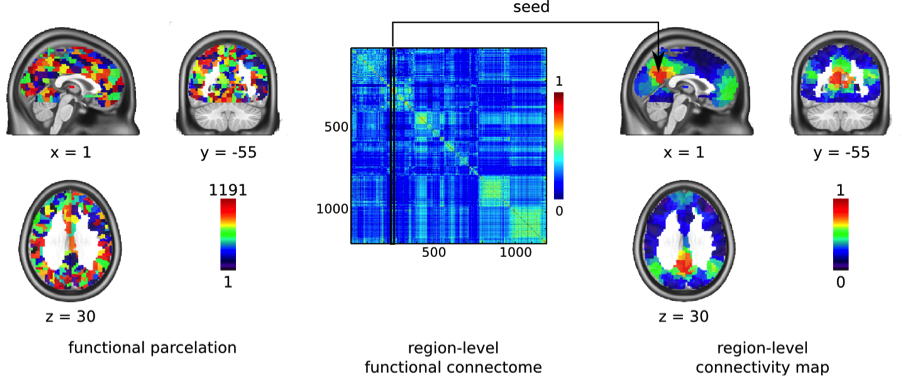
\includegraphics[width=\linewidth]{../figures/connectome.png}
\end{center}
\caption[Functional connectome]
{Functional connectome: on the left a representation of a functional parcellation, in the middle a region-level functional connectome representing the connectivity between each pair of region and on the right the connectivity map based on a region of interest extracted from the functional connectome.}
\label{fig_connectome}
\end{figure}

Several techniques have been used to identify these so-called resting-state networks (RSN). These networks show the functional organisation of various brain regions and several studies have demonstrated the relation of those functional networks to specific tasks in humans as well as in animal models \citep{Biswal1995} \citep{Buckner2008} \citep{Greicius2009}. Cordes et al. describe that several functional networks (sensorimotor, language and visual) identified in RS condition were exhibiting similar regions than the ones involved when performing a specific task (motor, language, or visual task) \citep{Cordes2000}. Based on such observations, CRSNs were then labeled according to the corresponding brain areas found active when performing such a specific task (e.g. motor or cognitive for example) thus associated with a brain function: e.g. auditory, visual, language networks \citep{Cordes2000} see Figure \ref{fig_crsn} for a list of common RSN. It enables us to establish the relationship between regions active 
when 
performing a specific task and RSNs, thus supporting the functional relevance of these networks. 


\begin{figure}[H]
\begin{center}
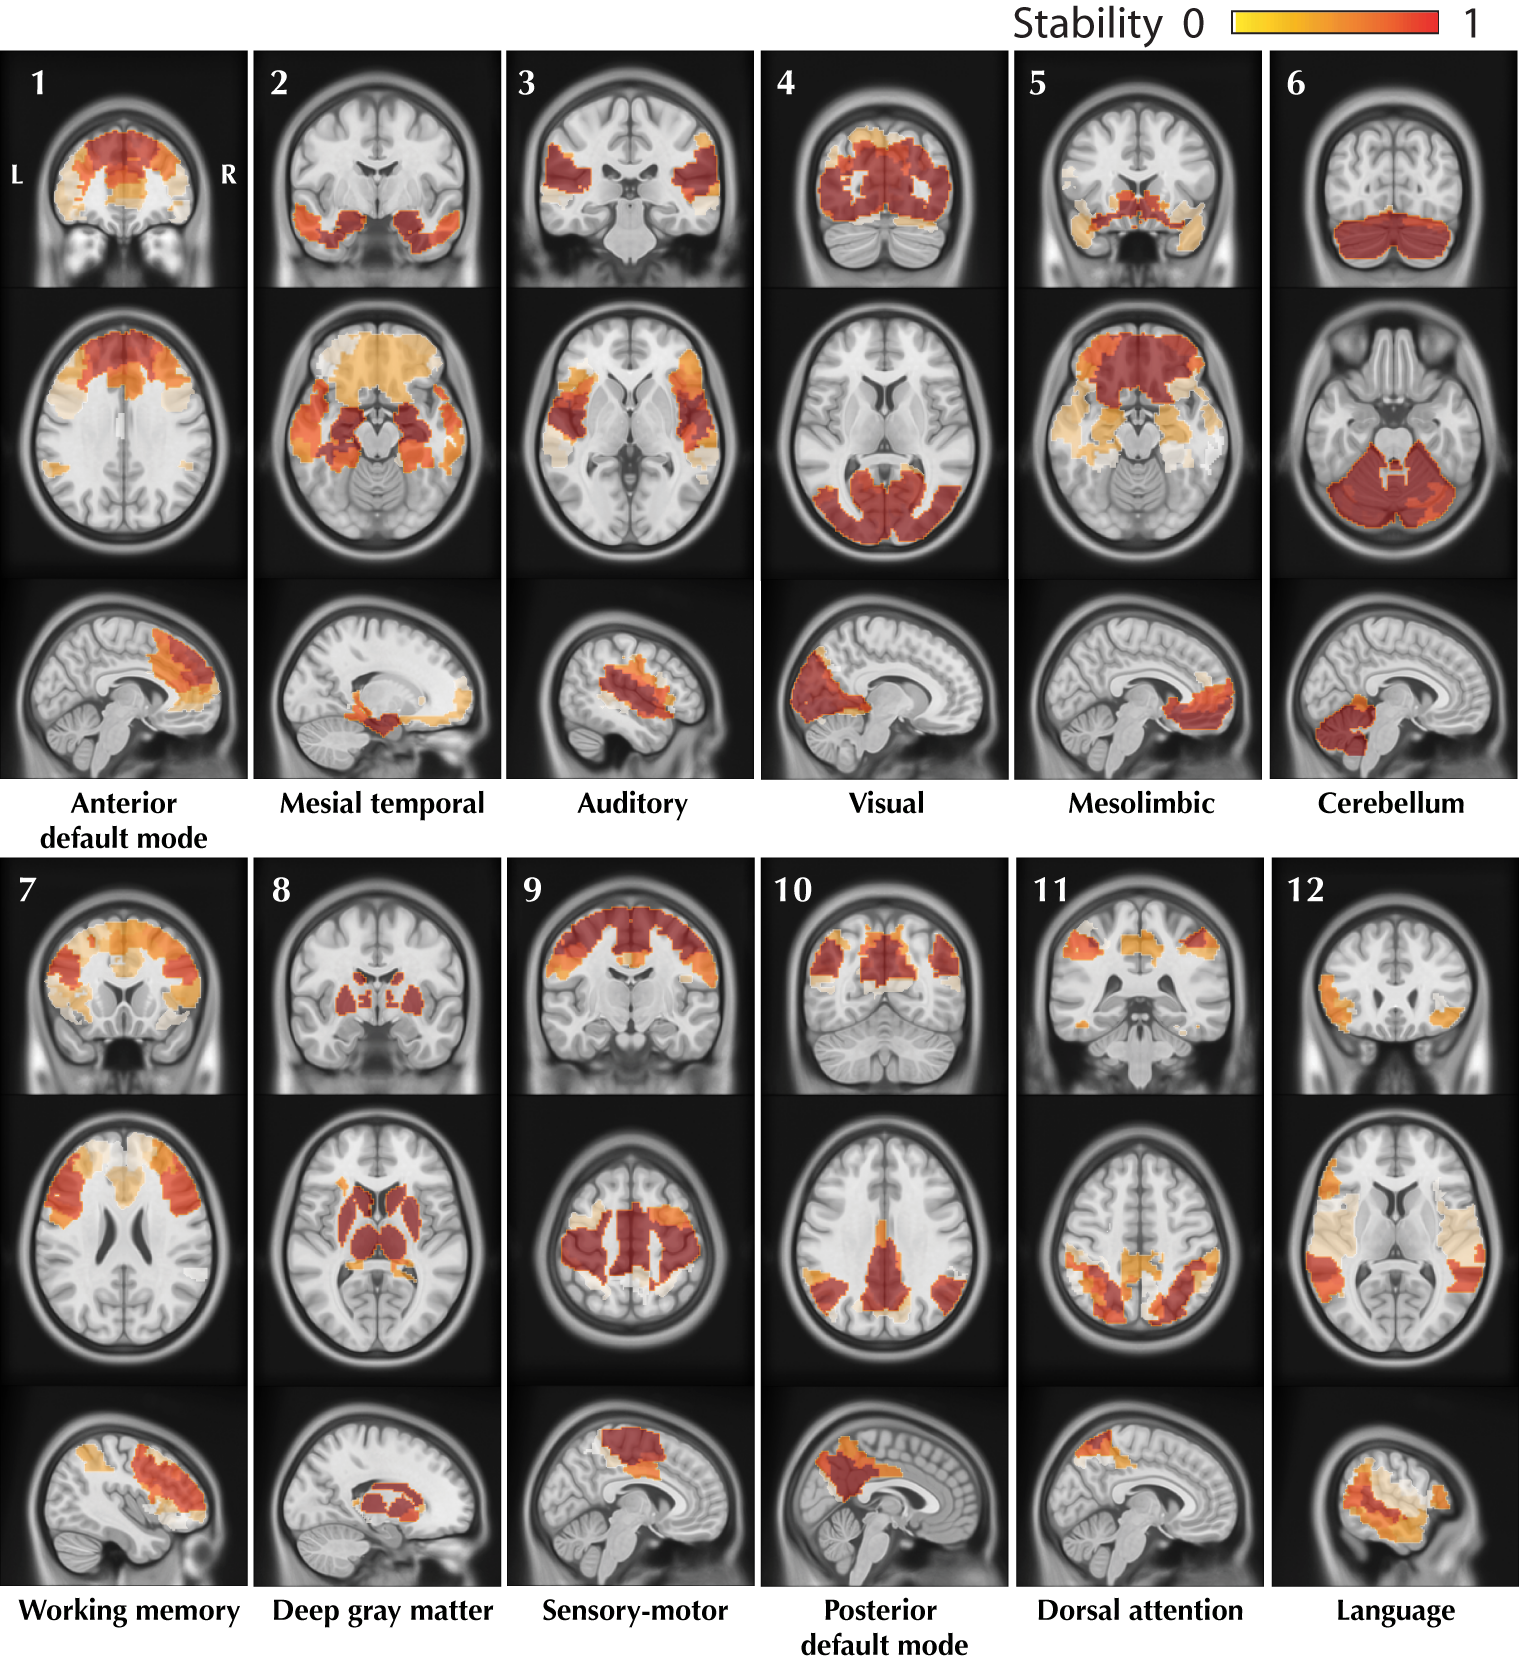
\includegraphics[scale=0.40]{../figures/CRSN.png}
\end{center}
\caption[Consistent resting-state network (CRSN)]
{The figure shows 12 CRSNs identified using BASC (Bootstrap Analysis of Stable Cluster \citep{Bellec2010c}) group level
analysis of 25 healthy control subjects. BASC is a clustering based method using evidence accumulation for the identification of stable cluster. For each CRSN: 3 slices (coronal, axial, sagittal)
are shown superimposed on an anatomical MRI template (MNI152). Labelling of each network was done visually based on previously reported CRSNs in the literature. The figure shows the usual networks: Default Mode Nettwork (\#1,\#10), Auditory (\#3), Visual (\#4), Sensory-Motor (\#9), Attention (\#7,\#11) and Language(\#12). BASC also identified 4 other networks, less often reported, but characterized by high statistical stability: Mesio-Temporal (\#2), Mesolimbic (\#5), Cerebellum (\#6) and Deep Gray Matter (\#8) \citep{Dansereau2014b} in press.}
\label{fig_crsn}
\end{figure}

Subsequently, rs-fMRI signal have been used in healthy subjects to investigate normal brain function, within various functional systems, such as auditory \citep{Cordes2001}, visual \citep{Lowe1998}, language \citep{Hampson2002}, limbic systems \citep{Greicius2003, Tian2007, Wink2006} and motor \citep{Jiang2004, Lowe1998}. Interestingly, resting-state fMRI signals have also been used to characterize the pathophysiological changes of some diseases, such as multiple sclerosis \citep{Lowe2002}, epilepsy \citep{Waites2006}, schizophrenia \citep{Liang2006, Salvador2007, Zhou2007, Zhou2008}, attention deficit hyperactivity disorder \citep{Tian2007, Zang2007}, blindness \citep{Liu2007, Yu2007}, major depression \citep{Anand2005, Greicius2007} and acute brainstem ischemia \citep{Salvador2005}. Thus, we believe that resting-state fMRI will be an increasingly important modality for exploring the functional abnormalities of patients with AD. Since a clinically meaningful hierarchical structure exist in the brain it is 
possible to use this structure to reduce the dimensionality of the problem and variability of the data while providing an informed organisation of the structure to a machine learning procedure looking to find functional markers characteristic of specific pathological populations (e.g. Alzheimer's disease).



\section{Prediction}
\subsection{Prediction in the context of AD}
In the past few years, several major studies have been initiated that have aimed to predict who will develop AD at the prodromal or even asymptomatic stage, with the ultimate goal of providing a platform for therapeutic intervention with disease-modifying therapies. Many of these studies were designed to evaluate the role of neuroimaging and chemical biomarkers in assessing and predicting progression in individuals without cognitive impairment and in individuals with MCI.
A very small literature currently reports findings on AD using rs-fMRI and they usually have outstanding performance like \citep{Jiang2014} ($94\%$). Unfortunately, the authors of this study performed a 10-fold cross-validation which did not include the feature selection process, which potentially lead to overestimation of the real accuracy. The rest of published studies have mainly used leave one out cross-validation and small sample size, which raises some concern with regards to the generalization ability of those trained predictors, e.g. \citep{Chen2011} ($87\%$), \citep{Dai2014} ($80\%$)).

\subsection{Importance of preprocessing to improve classification}
Preprocessing and normalization of the source data is a crucial point that may affect greatly the resulting classification or potential outcome measures. Moreover the introduction of multicentric data in the classification will render the task even more difficult, Nevertheless, a multi-site cohort helps test generalizability of the results across different samples, making it more likely that connections identified as predictive of a disease state indeed reflect generic traits of the pathology rather than particularities of a single dataset.

\subsection{High dimensionality problem}
In rs-fMRI, we obtain signal from brain activity at the voxel level representing more than $10^4$ voxels in the gray matter cortex, where the vast majority of the neurons are located. Although preprocessed, these data continue to have a lot of variance and we need to identify functional organisation more meaningful in term of clinical interpretation as well as an improved representation of the feature space that enhance the characterization of the functional modules. We can commonly extract functionally and clinically meaningful network features using principal component analysis (PCA) \citep{Zhong2009}, independent component analysis (ICA) \citep{McKeown1998}, various clustering algorithms such as k-means \citep{Baumgartner1998}, hierarchical clustering \citep{Cordes2002}, normalized cut-graph \citep{Heuvel2008}, self-organizing maps and neural gas \citep{Meyer-Baese2004}. Once we have functional parcels 
of the brain it is important to find the right metric to evaluate the connectivity between regions of the brain at the individual level. The most common metric use in the field of connectivity is the Pearson's correlation coefficient between the time series associated with a pair of regions.

\subsection{Feature selection}
Feature selection is often a critical step prior to any learning algorithm. The selection reduces the computational complexity of learning algorithms and exposes potentially clinically meaningful information. In many cases, this process can also improve the prediction accuracy by removing redundant and irrelevant information. Therefore feature selection is an important step in effective learning of large data sets. The features selection methods are usually organized into two categories: filter methods and wrapper methods \citep{Kotsiantis2007}. The filter method evaluates the relevance of features by looking only at the properties of the data without any knowledge on the classification labels. The wrapper method assesses the goodness a feature subset using the performance of a learning algorithm. The lack of reproducibility of reported markers (subset of features) is one of the main obstacle for the adoption of such marker in a clinical setup. If the marker is 
indeed discriminative of the pathology or of its progression we would expect the same features to be selected and exhibit similar performance across various studies. 

%relief proposed by xx is a feature selection method who try to optimise the margin between to class by selecting a sub sample of the features. An other algorithm called SIMBA proposed by algorithm proposed by Gilad-bachrach and colleagues in 2004 called margin based feature selection that aim to find the subset of features maximizing the margin between two classes.
%ensemble-based method \citep{Polikar2006} like Ada-boost to combine multiple week learners together

\subsection{Classification}
Machine learning methods have become very popular to classify functional brain images \citep{Costafreda2009,Fu2008,Hahn2011,Marquand2008,Nouretdinov2011}, for example to discriminate them between healthy and diseased populations. The most popular machine learning techniques in fMRI arguably is support vector machine (SVM) \citep{Cortes1995} which has been used in the past to categorize individual structural or functional brain images by differentiation of images from two groups (e.g. patient/control or male/female) \citep{Lao2004, Fan2005, Mourao-Miranda2005, Kawasaki2007}. 
%There is a modified version of SVM proposed by \cite{Li2011} called ccSVM who modify the kernel in order to account for confounding effects. 
A second widely used method is linear discriminant analysis (LDA) classifier; the main advantage of LDA is the ability to easily include confounding effects in the decision model, such as the inter-site difference in average connectivity measures.

\section{Objectives}
The objectives of the theses is to 1) reduce motion-related bias in connectivity measures, 2) evaluate the feasibility of multicentric fMRI analysis as well as identifying normalization procedures to reduce the between-site variance, and 3) design a prediction pipeline for the data-driven identification of biomarkers of AD in resting-state fMRI. The pipeline will have a feature selection tool to find a highly reduced set of functional connections with good prediction accuracy for the future conversion to a dementia of the Alzheimer's type in individuals with mild cognitive impairment.